% ju 17-Feb-24 Mars-Rover.tex
\documentclass{vorlage-design-main}
\usepackage[utf8]{inputenc}
\usepackage{longtable}
\usepackage{blindtext,alltt}
%% Ganze Überschrift
\title{Thema}

%% Kürzerer Titel zur Verwendung im Seitenkopf
\runningtitle{Kurztitel}
\author{Jan Unger}
% \author{2.}
\date{\today}

%% Die .bib-Datei mit vollständigen Referenzen zur Verwendung mit biblatex. articleclass lädt das Paket biblatex-chicago mit Anpassungen
\addbibresource{literatur.bib}

\begin{document}

\maketitle

\begin{abstract}

\end{abstract}

\begin{figure}
\centering
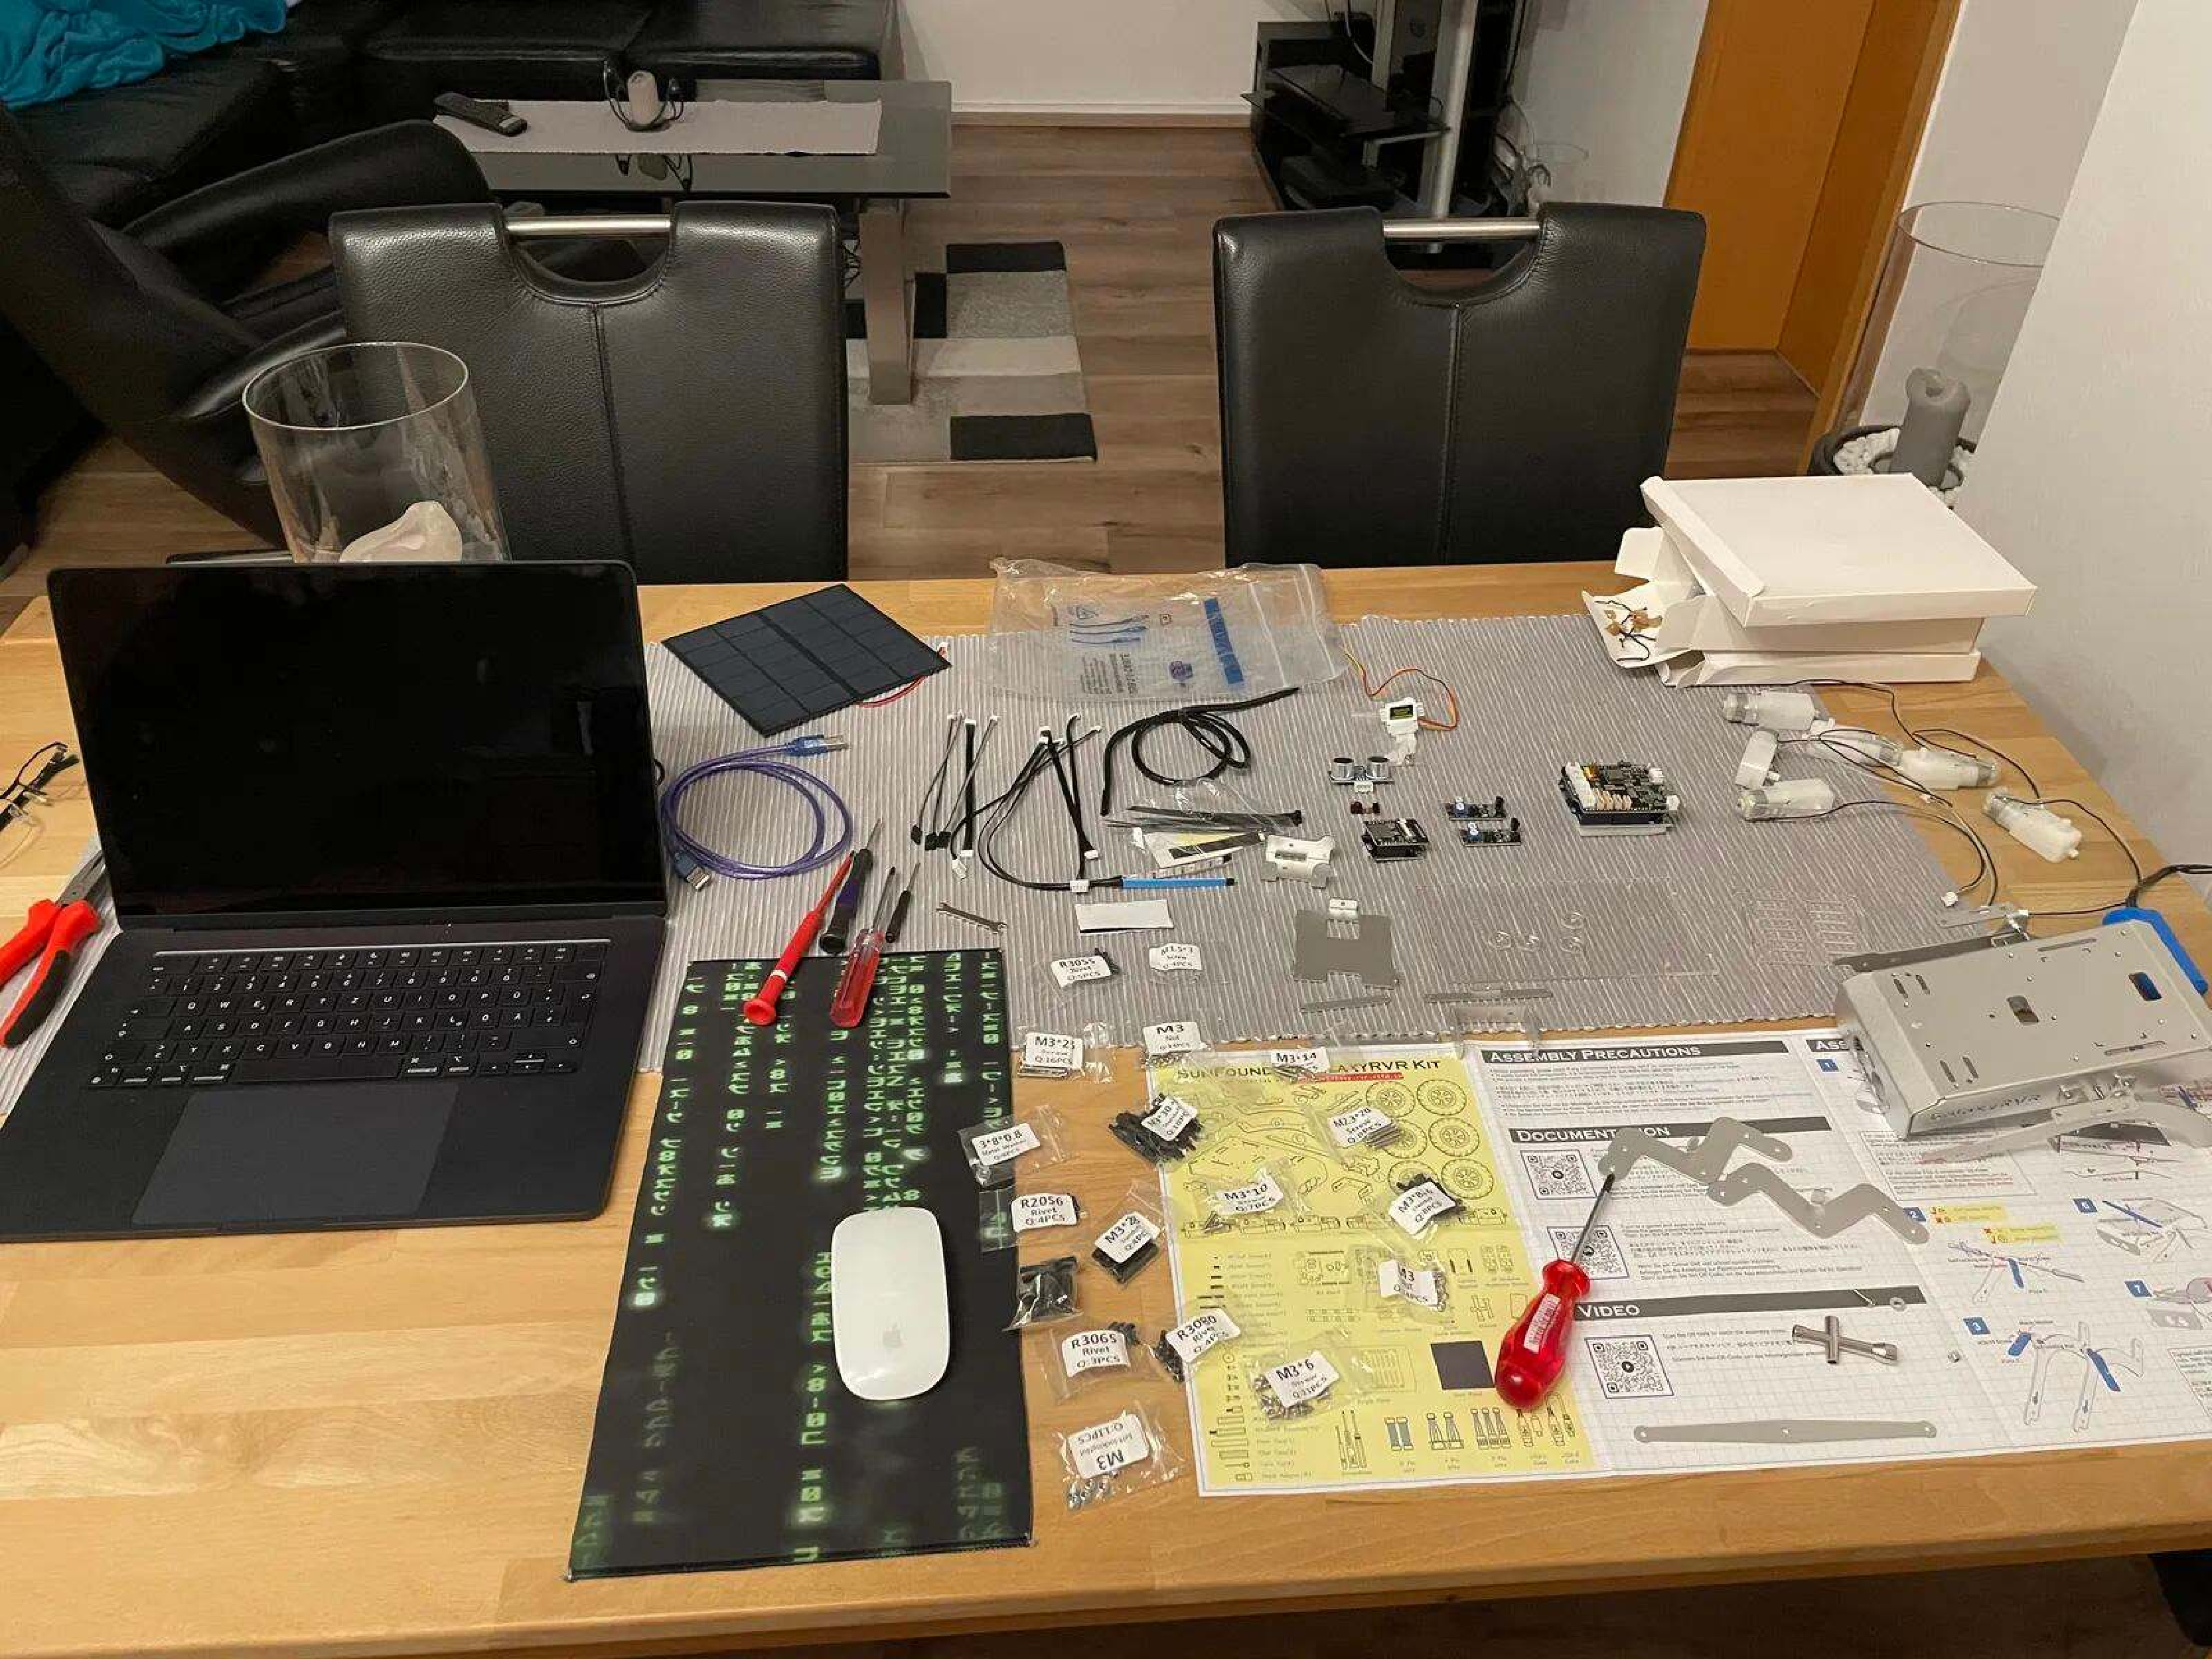
\includegraphics[width=0.8\textwidth]{images/rover-bau.pdf}
\floatnotes{}
%\label{fig:}
\caption{Mars-Rover Montage}
\end{figure}

\begin{figure}
\centering
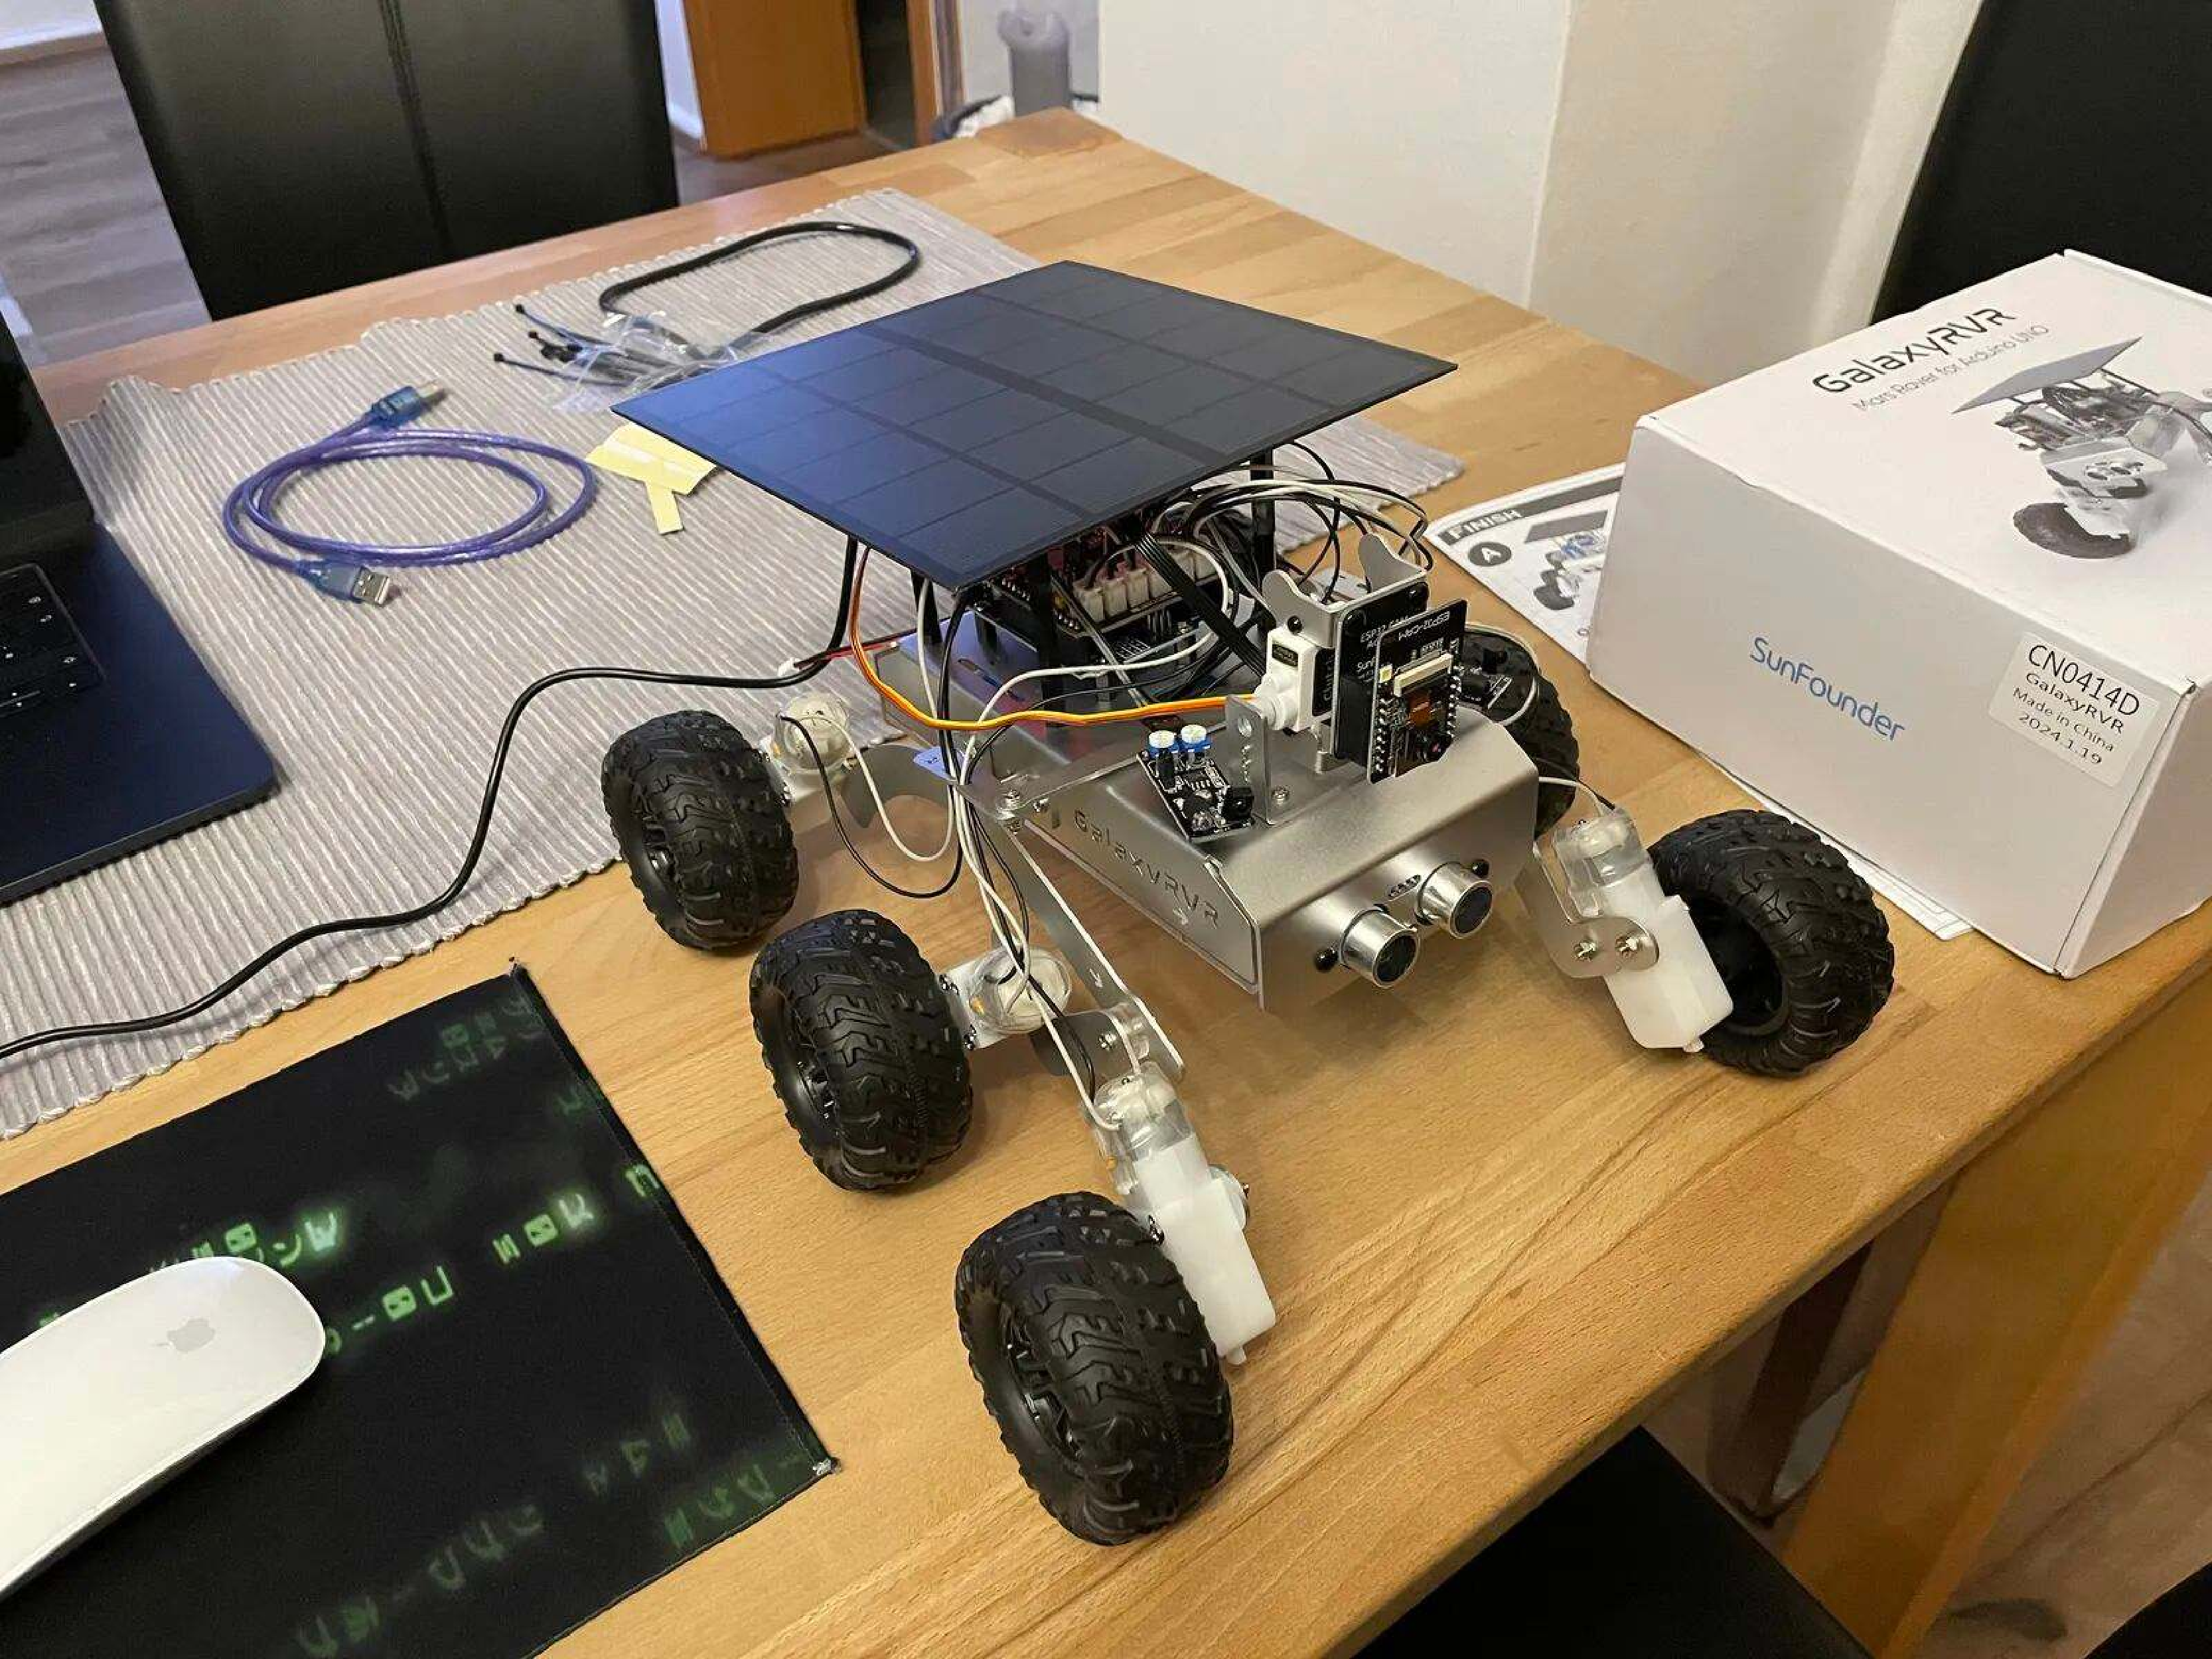
\includegraphics[width=0.8\textwidth]{images/rover-bau2.pdf}
\floatnotes{}
%\label{fig:}
\caption{Mars-Rover Montage 2}
\end{figure}

\hypertarget{enthuxfcllung-des-mars-rovers}{%
\subsection{Enthüllung des
Mars-Rovers}\label{enthuellung-des-mars-rovers}}

\hypertarget{unterschiede-in-den-designs}{%
\subsubsection{Unterschiede in den
Designs}\label{unterschiede-in-den-designs}}

\begin{itemize}

\item
  \textbf{Sojourner (1997)}: Als erster Rover auf dem Mars klein und
  relativ einfach gestaltet, mit dem Hauptziel, die Machbarkeit der
  Rover-Technologie auf dem Mars zu demonstrieren.
\item
  \textbf{Spirit und Opportunity (2004)}: Beide hatten ein
  ausgeklügelteres Design als Sojourner, waren größer, hatten eine
  längere Missionsdauer und waren mit fortschrittlicheren
  wissenschaftlichen Instrumenten ausgestattet, um Geologie und
  Atmosphäre zu erforschen.
\item
  \textbf{Curiosity (2012)}: Noch größer und komplexer, mit einem Labor
  an Bord, um chemische Analysen durchzuführen und nach Bedingungen für
  mikrobielles Leben zu suchen.
\item
  \textbf{Perseverance (2021)}: Baut auf Curiositys Design auf, mit
  zusätzlichen Instrumenten für astrobiologische Forschung,
  einschließlich der Suche nach fossilen Mikroben, und dem
  experimentellen Mars-Hubschrauber Ingenuity.
\end{itemize}

\hypertarget{gemeinsamkeiten}{%
\subsubsection{Gemeinsamkeiten}\label{gemeinsamkeiten}}

\begin{itemize}

\item
  Alle Rover sind mit Kameras und wissenschaftlichen Instrumenten
  ausgestattet, um den Mars zu studieren.
\item
  Solarenergie (bis Curiosity, der mit einem Radioisotopengenerator
  betrieben wird) und Kommunikationsfähigkeit mit der Erde.
\item
  Mobilität auf der Oberfläche zur Durchführung geologischer
  Untersuchungen und Atmosphärenmessungen.
\end{itemize}

\hypertarget{einfluss-der-missionsziele-auf-das-design}{%
\subsubsection{Einfluss der Missionsziele auf das
Design}\label{einfluss-der-missionsziele-auf-das-design}}

\begin{itemize}

\item
  Mit jedem Rover wuchsen die Missionsziele, was zu komplexeren Designs
  führte. Während Sojourner hauptsächlich die Technologie testete,
  suchten spätere Rover nach Wasserzeichen, aktuellen und vergangenen
  Lebensbedingungen und bereiteten die Mars-Erkundung durch Menschen
  vor.
\item
  Die Instrumentenauswahl reflektiert die spezifischen
  wissenschaftlichen Ziele jeder Mission.
\end{itemize}

\hypertarget{technologische-fortschritte}{%
\subsubsection{Technologische
Fortschritte}\label{technologische-fortschritte}}

\begin{itemize}

\item
  Fortschritte in der Robotik, Navigation, Energieversorgung und
  wissenschaftlichen Instrumentierung.
\item
  Von einfachen Kameras und Analyseinstrumenten zu hochauflösenden
  Kamerasystemen, Umweltsensoren, chemischen Analyseinstrumenten und dem
  ersten Fluggerät (Ingenuity).
\end{itemize}

\hypertarget{vorschluxe4ge-fuxfcr-den-nuxe4chsten-mars-rover}{%
\subsubsection{Vorschläge für den nächsten
Mars-Rover}\label{vorschlaege-fuer-den-naechsten-mars-rover}}

\begin{itemize}

\item
  Erweiterte Lebenssuche: Noch spezifischere Instrumente zur Detektion
  von Leben oder organischen Molekülen.
\item
  Probe-Return-Technologie: Integration von Systemen, um Proben für eine
  zukünftige Rückkehr zur Erde zu sammeln und zu konservieren.
\item
  Autonomie: Verbesserte autonome Navigationssysteme, um mehr Terrain
  sicher und effizient zu erkunden.
\item
  Technologien zur Unterstützung menschlicher Exploration: Experimente
  zur Ressourcengewinnung aus der Marsatmosphäre oder dem Boden.
\end{itemize}

\hypertarget{reflexionen-und-fragen}{%
\subsubsection{Reflexionen und Fragen}\label{reflexionen-und-fragen}}

\begin{itemize}

\item
  Wie können zukünftige Rover zur Vorbereitung menschlicher Missionen
  auf den Mars beitragen?
\item
  Welche neuen Technologien könnten zukünftige Rover revolutionieren?
\item
  Inwiefern können die gesammelten Daten dazu beitragen, die
  langfristige Bewohnbarkeit des Mars für Menschen zu verstehen?
\end{itemize}

\hypertarget{verstuxe4ndnis-und-bau-des-rocker-bogie-systems}{%
\subsection{Verständnis und Bau des
Rocker-Bogie-Systems}\label{verstaendnis-und-bau-des-rocker-bogie-systems}}

\begin{itemize}

\item
  \textbf{Einführung in das Rocker-Bogie-System}: Ein Federungssystem,
  das bei allen Mars-Rovern von Sojourner bis Perseverance verwendet
  wird, um eine optimale Anpassung an das raue Marsgelände zu
  gewährleisten.
\end{itemize}

\hypertarget{schritt-1-rocker-bogie-systems}{%
\subsubsection{Schritt 1:
Rocker-Bogie-Systems}\label{schritt-1-rocker-bogie-systems}}

\begin{itemize}

\item
  Das Rocker-Bogie-System ermöglicht es, dass alle Räder trotz unebener
  Oberflächen Bodenkontakt halten.
\item
  Zwei Hauptteile: >>Rocker<< (große Gliedmaßen für Bodenkontakt) und
  >>Bogie<< (kleineres Verbindungssystem für Flexibilität).
\end{itemize}

\hypertarget{schritt-2-system-in-aktion}{%
\subsubsection{Schritt 2: System in
Aktion}\label{schritt-2-system-in-aktion}}

\begin{itemize}
\item
  Warum denkst du, ist das Rocker-Bogie-Federungssystem für die
  Mars-Erkundung geeignet?
\item
  Kannst du beschreiben, wie das Rocker-Bogie-System in deinen eigenen
  Worten funktioniert?
\item
  Was sind die Schlüsselelemente des Rocker-Bogie-Systems, die den
  Rovern helfen, schwieriges Gelände zu bewältigen?
\end{itemize}

\hypertarget{schritt-3-bau-des-systems}{%
\subsubsection{Schritt 3: Bau des
Systems}\label{schritt-3-bau-des-systems}}

\begin{itemize}

\item
  Zusammenbau eines Rocker-Bogie-Systems mit einem GalaxyRVR-Kit und
  Diskussion seiner Komponenten.
\end{itemize}

\hypertarget{reflexion}{%
\subsubsection{Reflexion}\label{reflexion}}

Das Rocker-Bogie-Federungssystem ist für die Mars-Erkundung besonders
geeignet, da es eine außergewöhnliche Geländegängigkeit und Stabilität
bietet, die für die Bewältigung der unebenen und vielfältigen
Oberflächen des Mars unerlässlich sind. Dieses System ermöglicht es
Rovern, über große Steine und durch tiefe Sandgruben zu fahren, ohne
dass sie umkippen oder stecken bleiben, was bei der Erkundung eines
unbekannten und oft herausfordernden Terrains von entscheidender
Bedeutung ist.

Das Rocker-Bogie-System funktioniert auf eine Weise, die es dem Rover
ermöglicht, seine Räder unabhängig voneinander zu bewegen und sich an
die Oberfläche anzupassen, auf der er sich bewegt. Es besteht aus zwei
Teilen: dem >>Rocker<<, einem Gelenkarm, der sich auf einer Seite des
Rovers befindet, und dem >>Bogie<<, einem weiteren Gelenkarm auf der
gegenüberliegenden Seite. Diese Arme sind durch eine Querachse
miteinander verbunden, die dem System erlaubt, sich an Unebenheiten im
Gelände anzupassen, indem es die Gewichtsverteilung über die Räder
ausgleicht. Wenn ein Rad auf ein Hindernis trifft, können sich die
Rocker und Bogies so verstellen, dass alle Räder in Kontakt mit dem
Boden bleiben und der Rover stabilisiert wird.

Die Schlüsselelemente des Rocker-Bogie-Systems, die den Rovern helfen,
schwieriges Gelände zu bewältigen, umfassen:

\begin{enumerate}
\def\labelenumi{\arabic{enumi}.}

\item
  \textbf{Unabhängige Radbewegung}: Jedes Rad kann sich unabhängig
  voneinander heben oder senken, was es dem Rover ermöglicht, sich an
  die Geländeoberfläche anzupassen, über die er fährt.
\item
  \textbf{Gewichtsverteilung}: Das System verteilt das Gewicht des
  Rovers gleichmäßig auf alle Räder, was die Wahrscheinlichkeit eines
  Umkippens verringert und es dem Rover ermöglicht, über Hindernisse zu
  klettern, die größer sind als seine Räder.
\item
  \textbf{Anpassungsfähigkeit}: Die Rocker-Bogie-Konstruktion ermöglicht
  eine außerordentliche Flexibilität in der Bewegung, was dem Rover
  hilft, über komplexe Oberflächenstrukturen zu navigieren, ohne stecken
  zu bleiben oder beschädigt zu werden.
\end{enumerate}

\hypertarget{einstieg-in-die-welt-von-arduino-und-programmierung}{%
\subsection{Einstieg in die Welt von Arduino und
Programmierung¶}\label{einstieg-in-die-welt-von-arduino-und-programmierung}}

\begin{itemize}

\item
  \textbf{Arduino}:

  \begin{itemize}
  
  \item
    Eine benutzerfreundliche Open-Source-Plattform für Hardware und
    Software.
  \item
    Ermöglicht das Erstellen digitaler Geräte, die physische Vorgänge
    wahrnehmen und steuern können.
  \item
    Open-Source-Ansatz fördert Teilen und Kreativität.
  \end{itemize}
\item
  \textbf{Komponenten von Arduino}:

  \begin{itemize}
  
  \item
    \textbf{Mikrocontroller}: Das >>Gehirn<< von Arduino, ein kleiner
    Computer für einfache Aufgaben.
  \item
    \textbf{Entwicklungsboard}: Unterstützt den Mikrocontroller und
    enthält Komponenten für die Interaktion mit der Welt.
  \item
    \textbf{Arduino IDE}: Eine Entwicklungsumgebung, wo Anweisungen in
    C++ basierter Sprache geschrieben werden, um dem Arduino Befehle zu
    erteilen.
  \end{itemize}
\item
  \textbf{SunFounder R3 Board}:

  \begin{itemize}
  
  \item
    Ein spezifisches Arduino-kompatibles Board mit zahlreichen
    Funktionen für Projektentwicklungen.
  \item
    Verfügt über 14 digitale Pins für Eingabe/Ausgabe-Aktionen und 6
    analoge Pins zur Sensorintegration.
  \item
    USB-Anschluss für die Programmübertragung und ein Power Jack für die
    Stromversorgung.
  \item
    ICSP Header für externe Programmierer und einen Reset-Button zum
    Neustarten des Programms.
  \end{itemize}
\item
  \textbf{Arduino-Programmierung}:

  \begin{itemize}
  
  \item
    \textbf{Grundlegende Funktionen}:

    \begin{itemize}
    
    \item
      \verb|setup()|: Initialisiert Variablen,
      Pin-Modi etc., wird einmal zu Beginn ausgeführt.
    \item
      \verb|loop()|: Enthält den Code, der wiederholt
      ausgeführt wird (Hauptschleife).
    \item
      \verb|pinMode()|: Definiert Pins als Eingang
      oder Ausgang.
    \item
      \verb|digitalWrite()|: Setzt den Pin auf HIGH
      oder LOW.
    \item
      \verb|delay()|: Pausiert das Programm für eine
      angegebene Zeit.
    \end{itemize}
  \end{itemize}
\end{itemize}

\hypertarget{beherrschung-des-tt-motors}{%
\subsection{Beherrschung des
TT-Motors}\label{beherrschung-des-tt-motors}}

\begin{itemize}

\item
  \textbf{Grundlagen von Motoren}:

  \begin{itemize}
  
  \item
    Ein Motor wandelt elektrische in mechanische Energie um, basierend
    auf dem Prinzip der elektromagnetischen Induktion.
  \item
    Der TT-Motor, ein Getriebemotor in einem Kunststoffgehäuse, erhöht
    durch Zahnräder das Drehmoment für effektive Bewegungen.
  \end{itemize}
\item
  \textbf{Steuerung von Motoren}:

  \begin{itemize}
  
  \item
    Direktes Anschließen eines Motors an eine Batterie führt zur
    Drehung; die Umkehr der Anschlüsse ändert die Drehrichtung.
  \item
    Arduino-Boards allein reichen nicht aus, um Motoren zu betreiben, da
    deren Signalpins nicht genügend Strom liefern.
  \item
    Motor-Treiber dienen als Verstärker zwischen Arduino und Motor, um
    Bewegungen zu steuern.
  \end{itemize}
\item
  \textbf{Einsatz des GalaxyRVR-Shields}:

  \begin{itemize}
  
  \item
    Das Shield dient als Schnittstelle für die Steuerung von bis zu
    sechs Motoren und verbindet Sensoren sowie Stromversorgung.
  \item
    Die Steuerung erfolgt über spezifische Pins, die an
    Motor-Treiber-Chips angeschlossen sind, welche die Motoren
    aktivieren.
  \end{itemize}
\item
  \textbf{Programmierung zur Motorsteuerung}:

  \begin{itemize}
  
  \item
    Grundlegende Befehle (wie \verb|digitalWrite()|
    und \verb|pinMode()|) steuern Richtung und
    Aktivität des Motors.
  \item
    Die Anwendung der Pulsweitenmodulation (PWM) ermöglicht die
    Feinabstimmung der Motorgeschwindigkeit.
  \item
    Arduino-Bibliotheken wie SoftPWM erweitern die Möglichkeiten zur
    Geschwindigkeitskontrolle durch Software.
  \end{itemize}
\end{itemize}

\hypertarget{antriebslogik}{%
\subsubsection{Antriebslogik}\label{antriebslogik}}

\begin{table}[!ht]
\caption{}% \label{tab:}%% anpassen
\begin{tabular}{@{}ccl@{}}

\toprule
INA & INB & Motor \\
\midrule[\heavyrulewidth]

L & L & Standby \\
L & H & Im Uhrzeigersinn \\
H & L & Gegen den Uhrzeigersinn \\
H & H & Bremse \\
\bottomrule

\end{tabular}
\floatnotes{}
\end{table}

Treiberchips mit den Pins 2, 3, 4 und 5 und verwenden die
SoftPWM-Bibliothek von Arduino, um PWM auf diesen Pins zu ermöglichen.

\begin{lstlisting}[language={C++}]
// Wie würdest du den Code ändern, um sechs Motoren gleichzeitig zu steuern?
const int in3 = 4;
const int in4 = 5;

void setup() {
    pinMode(in3, OUTPUT);
    pinMode(in4, OUTPUT);
}

void loop() {
    digitalWrite(in3, LOW);
    digitalWrite(in4, HIGH);
    delay(2000);
    digitalWrite(in3, HIGH);
    digitalWrite(in4, LOW);
    delay(2000);
    digitalWrite(in3, HIGH);
    digitalWrite(in4, HIGH);
    delay(5000);
}
\end{lstlisting}

\begin{lstlisting}[language={C++}]
Um sechs Motoren gleichzeitig zu steuern und dabei die Antriebslogik sowie die Nutzung der SoftPWM-Bibliothek für das Arduino-Board zu berücksichtigen, muss der vorgegebene Code erweitert werden. Da die Pins 2 und 3 für die Steuerung der Motoren A, B, C und die Pins 4 und 5 für die Steuerung der Motoren D, E, F verwendet werden, kann der Code wie folgt angepasst werden, um alle sechs Motoren gleichzeitig zu steuern:

>>`c++
#include <SoftPWM.h>

// Definition der Pins für die Motoren A, B, C
const int motorA1 = 2; // INA für Motoren A, B, C
const int motorA2 = 3; // INB für Motoren A, B, C

// Definition der Pins für die Motoren D, E, F
const int motorB1 = 4; // INA für Motoren D, E, F
const int motorB2 = 5; // INB für Motoren D, E, F

void setup() {
    // Initialisierung der Pins als Ausgang
    SoftPWMBegin(); // Start der SoftPWM-Bibliothek
    
    pinMode(motorA1, OUTPUT);
    pinMode(motorA2, OUTPUT);
    pinMode(motorB1, OUTPUT);
    pinMode(motorB2, OUTPUT);

    // Setzt die PWM-Auflösung für die Pins
    SoftPWMSet(motorA1, 0);
    SoftPWMSet(motorA2, 0);
    SoftPWMSet(motorB1, 0);
    SoftPWMSet(motorB2, 0);
}

void loop() {
    // Motoren A, B, C im Uhrzeigersinn
    SoftPWMSet(motorA1, LOW);
    SoftPWMSet(motorA2, HIGH);
    
    // Motoren D, E, F im Uhrzeigersinn
    SoftPWMSet(motorB1, LOW);
    SoftPWMSet(motorB2, HIGH);
    
    delay(2000); // Wartezeit
    
    // Motoren A, B, C gegen den Uhrzeigersinn
    SoftPWMSet(motorA1, HIGH);
    SoftPWMSet(motorA2, LOW);
    
    // Motoren D, E, F gegen den Uhrzeigersinn
    SoftPWMSet(motorB1, HIGH);
    SoftPWMSet(motorB2, LOW);
    
    delay(2000); // Wartezeit
    
    // Alle Motoren stoppen (Bremse)
    SoftPWMSet(motorA1, HIGH);
    SoftPWMSet(motorA2, HIGH);
    SoftPWMSet(motorB1, HIGH);
    SoftPWMSet(motorB2, HIGH);
    
    delay(5000); // Wartezeit
}
\end{lstlisting}

Dieser Code nutzt die SoftPWM-Bibliothek, um PWM-Signale auf den Pins 2,
3, 4 und 5 zu ermöglichen, was eine feinere Kontrolle über die
Motorgeschwindigkeit erlaubt. Die Antriebslogik wird beibehalten, indem
die Pins in verschiedenen Kombinationen (LOW/HIGH) gesetzt werden, um
die Motoren in unterschiedliche Richtungen zu drehen oder sie zu
stoppen. Durch die parallele Anbindung der Motoren an jeweils zwei Pins
können alle sechs Motoren simultan gesteuert werden, was eine flexible
und effektive Kontrolle des Systems ermöglicht.

\begin{lstlisting}
### Steuerung der Motorgeschwindigkeit (PWM)

>>`c++
// Steuerung der Motorgeschwindigkeit
// SoftPWM, for-Schleife
#include <SoftPWM.h>

const int in1 = 2;
const int in2 = 3;

void setup() {
    SoftPWMBegin();
}

void loop() {
    SoftPWMSet(in1, 0);
    for (int i = 0; i <= 255; i++) {
        SoftPWMSet(in2, i);
        delay(100);
}
    delay(1000);
}
\end{lstlisting}

Pulsweitenmodulation (PWM) mit der SoftPWM-Bibliothek in Arduino
verwendet wird, um die Geschwindigkeit eines Motors zu steuern. Die
SoftPWM-Bibliothek ermöglicht es, PWM auf digitalen Pins zu simulieren,
die keine nativen PWM-Fähigkeiten haben. Der Code durchläuft einen
Zyklus, bei dem die Geschwindigkeit des Motors schrittweise von 0 bis
zum Maximum erhöht wird.

\begin{lstlisting}[language={C++}]
#include <SoftPWM.h>

const int in1 = 2;
const int in2 = 3;

void setup() {
    SoftPWMBegin();
    SoftPWMSet(in1, 0);
}

void loop() {
    // Geschwindigkeit erhöhen
    for (int i = 0; i <= 255; i++) {
        SoftPWMSet(in2, i);
        delay(20); // Schnellere Änderung der Geschwindigkeit
    }
    
    delay(1000); // Kurze Pause bei maximaler Geschwindigkeit

    // Geschwindigkeit verringern
    for (int i = 255; i >= 0; i--) {
        SoftPWMSet(in2, i);
        delay(20); // Schnellere Änderung der Geschwindigkeit
    }

    delay(1000); // Kurze Pause bei minimaler Geschwindigkeit
}
\end{lstlisting}

Hardware-PWM (Pulsweitenmodulation) und Software-PWM (z.B. mit der
SoftPWM-Bibliothek für Arduino) bieten beide die Möglichkeit, die
Ausgangsleistung an einem Pin zu steuern, unterscheiden sich jedoch in
ihrer Implementierung und Leistungsfähigkeit.

\hypertarget{unterschiede-zwischen-hardware-pwm-und-software-pwm}{%
\subsubsection{Unterschiede zwischen Hardware-PWM und
Software-PWM}\label{unterschiede-zwischen-hardware-pwm-und-software-pwm}}

\begin{itemize}

\item
  \textbf{Hardware-PWM}:

  \begin{itemize}
  
  \item
    Wird direkt von den Mikrocontroller-Hardwareeinheiten
    bereitgestellt.
  \item
    Bietet eine präzisere und stabilere PWM-Signalgenerierung im
    Vergleich zu Software-PWM, da sie nicht von der CPU-Auslastung oder
    Software-Verzögerungen beeinflusst wird.
  \item
    Die Anzahl der verfügbaren Hardware-PWM-Pins ist begrenzt und hängt
    vom spezifischen Mikrocontroller ab.
  \item
    Ermöglicht in der Regel höhere Frequenzen und eine bessere Auflösung
    des PWM-Signals.
  \end{itemize}
\item
  \textbf{Software-PWM}:

  \begin{itemize}
  
  \item
    Wird durch Software-Algorithmen realisiert, die auf beliebigen
    digitalen Pins ausgeführt werden können.
  \item
    Kann flexibler sein, da nahezu jeder Pin als PWM-Ausgang verwendet
    werden kann, ist aber weniger präzise und kann durch andere Vorgänge
    im Programm beeinträchtigt werden.
  \item
    Die Frequenz und Auflösung des PWM-Signals kann durch die
    Prozessorgeschwindigkeit und die Effizienz der
    Software-Implementierung begrenzt sein.
  \item
    Kann mehr CPU-Ressourcen verbrauchen, was die Leistung anderer Teile
    des Programms beeinträchtigen kann.
  \end{itemize}
\end{itemize}

\hypertarget{beispiel-fuxfcr-hardware-pwm-mit-arduino}{%
\subsubsection{Beispiel für Hardware-PWM mit
Arduino}\label{beispiel-fuer-hardware-pwm-mit-arduino}}

Steuerung der Helligkeit einer LED. Die Arduino-Boards haben Pins, mit
einem Tilde-Symbol (\textasciitilde{} Pins 3, 5, 6, 9, 10 und 11 auf dem
Arduino Uno).

\begin{lstlisting}[language={C++}]
int ledPin = 9; // Pin mit Hardware-PWM-Funktion

void setup() {
  pinMode(ledPin, OUTPUT);
}

void loop() {
  for (int i = 0; i <= 255; i++) {
    analogWrite(ledPin, i); // Setzt die Helligkeit der LED
    delay(10);
  }
  
  for (int i = 255; i >= 0; i--) {
    analogWrite(ledPin, i); // Verringert die Helligkeit der LED
    delay(10);
  }
}
\end{lstlisting}

\hypertarget{reflektieren-und-verbessern}{%
\subsubsection{Reflektieren und
Verbessern}\label{reflektieren-und-verbessern}}

\begin{itemize}
\item
  Arbeitsprinzipien von Motoren

  \begin{itemize}
  
  \item
    Motor das Prinzip der elektromagnetischen Induktionegen.
  \item
    TT-Getriebemotor
  \end{itemize}
\item
  Wie steuert man ihre Richtung und Geschwindigkeit durch
  Programmierung.
\item
  Wie würdest du die for-Schleife ändern, um die Motorgeschwindigkeit
  allmählich zu verringern?
\item
  Wie würdest du den Motor so steuern, dass er beim Drehen gegen den
  Uhrzeigersinn beschleunigt oder verlangsamt?
\end{itemize}

\hypertarget{arbeitsprinzipien-von-motoren}{%
\subsubsection{Arbeitsprinzipien von
Motoren}\label{arbeitsprinzipien-von-motoren}}

\begin{itemize}

\item
  \textbf{Elektromagnetische Induktion}: Die Drehbewegung eines Motors
  entsteht durch die Interaktion eines erzeugten Magnetfelds mit den
  Magneten im Motor. Dieses Prinzip ermöglicht es, elektrische Energie
  in mechanische Bewegung umzuwandeln.
\item
  \textbf{TT-Getriebemotor}: Die Kombination aus Motor und Getriebe in
  einem TT-Getriebemotor ermöglicht es, das Drehmoment zu erhöhen.
  Dadurch kann der Motor größere Lasten bewegen, was ihn ideal für
  Anwendungen wie Rover auf unebenem Terrain macht.
\end{itemize}

\hypertarget{steuerung-der-richtung-und-geschwindigkeit-durch-programmierung}{%
\subsubsection{Steuerung der Richtung und Geschwindigkeit durch
Programmierung}\label{steuerung-der-richtung-und-geschwindigkeit-durch-programmierung}}

\begin{itemize}

\item
  \textbf{Richtungssteuerung}: Die Richtung eines Motors wird durch
  Ändern der Polarität der an den Motor angelegten Spannung bestimmt. In
  einem Programm kann dies durch Wechseln der HIGH/LOW-Zustände der Pins
  erreicht werden, die den Motor steuern.
\item
  \textbf{Geschwindigkeitssteuerung}: Die Geschwindigkeit eines Motors
  kann durch Pulsweitenmodulation (PWM) angepasst werden, wobei die
  durchschnittliche Spannung, die dem Motor zugeführt wird, durch Ändern
  des Tastverhältnisses des PWM-Signals variiert wird.
\end{itemize}

\hypertarget{programmierbeispiele}{%
\subsubsection{Programmierbeispiele}\label{programmierbeispiele}}

\hypertarget{motorgeschwindigkeit-allmuxe4hlich-verringern}{%
\paragraph{Motorgeschwindigkeit allmählich
verringern}\label{motorgeschwindigkeit-allmaehlich-verringern}}

Um die Motorgeschwindigkeit allmählich zu verringern, kann man eine
\verb|for|-Schleife verwenden, die den PWM-Wert von
einem hohen Wert schrittweise auf einen niedrigeren Wert reduziert:

\begin{lstlisting}[language={C++}]
for (int i = 255; i >= 0; i--) {
    analogWrite(motorPin, i);
    delay(20); // Verzögerung für sichtbare Geschwindigkeitsänderung
}
\end{lstlisting}

\hypertarget{motor-beschleunigenverlangsamen-gegen-den-uhrzeigersinn}{%
\paragraph{Motor beschleunigen/verlangsamen gegen den
Uhrzeigersinn}\label{motor-beschleunigenverlangsamen-gegen-den-uhrzeigersinn}}

Die Beschleunigung oder Verlangsamung eines Motors in eine bestimmte
Richtung, wie gegen den Uhrzeigersinn, erfordert die Steuerung der
Drehrichtung sowie die Anpassung der Geschwindigkeit. Dies kann durch
Kombination der Richtungssteuerung und schrittweise Anpassung des
PWM-Werts erreicht werden:

\begin{lstlisting}[language={C++}]
// Setzt die Richtung auf gegen den Uhrzeigersinn
digitalWrite(directionPin1, HIGH);
digitalWrite(directionPin2, LOW);

// Beschleunigung
for (int i = 0; i <= 255; i++) {
    analogWrite(speedPin, i);
    delay(20);
}

// Kurze Pause
delay(1000);

// Verlangsamung
for (int i = 255; i >= 0; i--) {
    analogWrite(speedPin, i);
    delay(20);
}
\end{lstlisting}

\hypertarget{entfesselung-der-beweglichkeit-des-mars-rovers}{%
\subsection{Entfesselung der Beweglichkeit des Mars
Rovers¶}\label{entfesselung-der-beweglichkeit-des-mars-rovers}}

\begin{itemize}

\item
  \textbf{Integration von Motoren ins Rocker-Bogie-System}: Das
  Rocker-Bogie-System ist speziell für die Bewältigung der komplexen und
  unebenen Marslandschaften konzipiert. Die Einbindung von TT-Motoren in
  dieses System erweitert dessen Fähigkeit, sich an diverse Geländearten
  anzupassen, indem es eine verbesserte Mobilität und Stabilität bietet.
\item
  \textbf{Programmierung des Mars Rovers}: Die Verwendung der
  Arduino-Plattform ermöglicht eine präzise Steuerung der Motoren, was
  die Grundlage für die Bewegungskontrolle des Rovers bildet. Die
  Programmierung umfasst die Steuerung der Motordrehrichtung und
  -geschwindigkeit, um Vorwärts-, Rückwärts- und Drehbewegungen zu
  realisieren.
\end{itemize}

\hypertarget{implementierungsschritte}{%
\subsubsection{Implementierungsschritte}\label{implementierungsschritte}}

\begin{enumerate}
\def\labelenumi{\arabic{enumi}.}

\item
  \textbf{Bewegungssteuerung}: Durch Programmierung werden die Motoren
  so angesteuert, dass der Rover vorwärts und rückwärts fahren sowie
  nach links und rechts drehen kann. Dies wird durch Anpassung der
  Drehrichtung und Geschwindigkeit der Motoren erreicht.
\item
  \textbf{Programmbeispiele}: Die Bereitstellung von Codebeispielen
  illustriert, wie die SoftPWM-Bibliothek genutzt wird, um die
  Geschwindigkeit und Richtung der Motoren feinabzustimmen. Die
  Variation der PWM-Werte ermöglicht es, die Geschwindigkeit der Motoren
  dynamisch anzupassen, was eine differenzierte Steuerung der Bewegung
  des Rovers ermöglicht.
\item
  \textbf{Erweiterung der Bewegungssteuerung}: Die Entwicklung von
  Funktionen für spezifische Bewegungsabläufe erleichtert die
  Programmstrukturierung und erhöht die Wiederverwendbarkeit des Codes.
  Durch diese Modularisierung wird der Code nicht nur übersichtlicher,
  sondern auch flexibler für zukünftige Anpassungen und Erweiterungen.
\end{enumerate}

\hypertarget{den-rover-in-bewegung-setzen}{%
\subsubsection{Den Rover in Bewegung
setzen}\label{den-rover-in-bewegung-setzen}}

\hypertarget{rover-vorwuxe4rts-bewegen}{%
\paragraph{Rover vorwärts bewegen}\label{rover-vorwaerts-bewegen}}

\begin{itemize}

\item
  \textbf{Initialisierung}: Die SoftPWM-Bibliothek wird initialisiert,
  was es ermöglicht, PWM-Signale auf den Pins
  \verb|in1|, \verb|in2|,
  \verb|in3|, und \verb|in4| zu
  generieren.
\item
  \textbf{Motorsteuerung}:

  \begin{itemize}
  
  \item
    Die linken Motoren (\verb|in1| und
    \verb|in2|) werden so gesteuert, dass
    \verb|in1| auf volle Geschwindigkeit gesetzt wird
    (255), während \verb|in2| gestoppt wird (0). Dies
    bewirkt, dass die linken Motoren gegen den Uhrzeigersinn drehen.
  \item
    Gleichzeitig werden die rechten Motoren
    (\verb|in3| und \verb|in4|) so
    gesteuert, dass \verb|in3| gestoppt wird (0) und
    \verb|in4| auf volle Geschwindigkeit gesetzt wird
    (255), was zu einer Drehung im Uhrzeigersinn führt.
  \end{itemize}
\item
  \textbf{Ergebnis}: Durch diese Konfiguration der Motorsteuerung bewegt
  sich der Rover vorwärts, da die gegenüberliegenden Seiten des Rovers
  in entgegengesetzte Richtungen drehen, wodurch Vorwärtsbewegung
  entsteht.
\end{itemize}

\begin{lstlisting}[language={C++}]
// Rover vorwärts bewegen
#include <SoftPWM.h>

// Definiert die Pins für die Motoren
const int in1 = 2;
const int in2 = 3;
const int in3 = 4;
const int in4 = 5;

/*
 * Initialisiert das Programm und die SoftPWM-Bibliothek.
 * Dieser Teil des Codes wird einmal beim Start des Programms ausgeführt.
 */
void setup() {
    // Initialisiert die SoftPWM-Bibliothek
    SoftPWMBegin();
}

/*
 * Hauptteil des Programms, der kontinuierlich ausgeführt wird.
 * Hier wird die Bewegung der Motoren gesteuert, um den Rover vorwärts zu bewegen.
 */
void loop() {
    // Setzt die linken Motoren so, dass sie gegen den Uhrzeigersinn drehen
    SoftPWMSet(in1, 255);  // Volle Geschwindigkeit
    SoftPWMSet(in2, 0);    // Stop

    // Setzt die rechten Motoren so, dass sie im Uhrzeigersinn drehen
    SoftPWMSet(in3, 0);    // Stop
    SoftPWMSet(in4, 255);  // Volle Geschwindigkeit
}
\end{lstlisting}

\hypertarget{rover-ruxfcckwuxe4rts-bewegen}{%
\paragraph{Rover rückwärts
bewegen}\label{rover-rueckwaerts-bewegen}}

\begin{itemize}

\item
  \textbf{Initialisierung}: Wie im ersten Beispiel wird die
  SoftPWM-Bibliothek initialisiert.
\item
  \textbf{Motorsteuerung}:

  \begin{itemize}
  
  \item
    Die Steuerung der linken Motoren (\verb|in1| und
    \verb|in2|) wird umgekehrt, indem
    \verb|in1| gestoppt wird (0) und
    \verb|in2| auf volle Geschwindigkeit gesetzt wird
    (255), was eine Drehung im Uhrzeigersinn bewirkt.
  \item
    Für die rechten Motoren (\verb|in3| und
    \verb|in4|) wird \verb|in3|
    auf volle Geschwindigkeit gesetzt (255) und
    \verb|in4| gestoppt (0), was eine Drehung gegen
    den Uhrzeigersinn zur Folge hat.
  \end{itemize}
\item
  \textbf{Ergebnis}: Diese Anordnung führt dazu, dass der Rover sich
  rückwärts bewegt, da die Motoren auf beiden Seiten des Rovers in
  umgekehrter Richtung zur Vorwärtsbewegung drehen.
\end{itemize}

\begin{lstlisting}[language={C++}]
// Rover rückwärts bewegen
#include <SoftPWM.h>

// Definiert die Pins für die Motoren
const int in1 = 2;
const int in2 = 3;
const int in3 = 4;
const int in4 = 5;

/*
 * Initialisiert das Programm und die SoftPWM-Bibliothek.
 * Dieser Teil des Codes wird einmal beim Start des Programms ausgeführt.
 */
void setup() {
    // Initialisiert die SoftPWM-Bibliothek
    SoftPWMBegin();
}

/*
 * Hauptteil des Programms, der kontinuierlich ausgeführt wird.
 * Hier wird die Bewegung der Motoren gesteuert, um den Rover rückwärts zu bewegen.
 */
void loop() {
    // Setzt die linken Motoren so, dass sie im Uhrzeigersinn drehen
    SoftPWMSet(in1, 0);    // Stop
    SoftPWMSet(in2, 255);  // Volle Geschwindigkeit

    // Setzt die rechten Motoren so, dass sie gegen den Uhrzeigersinn drehen
    SoftPWMSet(in3, 255);  // Volle Geschwindigkeit
    SoftPWMSet(in4, 0);    // Stop
}
\end{lstlisting}

\hypertarget{rover-in-andere-richtungen-bewegen}{%
\subsubsection{Rover in andere Richtungen
bewegen}\label{rover-in-andere-richtungen-bewegen}}

\begin{enumerate}
\def\labelenumi{\arabic{enumi}.}
\item
  Methode besteht darin, die Räder auf der linken Seite langsamer als
  die auf der rechten Seite rotieren zu lassen. Dieser
  Geschwindigkeitsunterschied wird den Rover nach links abbiegen lassen.
\item
  Methode besteht darin, beide linken und rechten Motoren in dieselbe
  Richtung rotieren zu lassen (in diesem Fall im Uhrzeigersinn), was den
  Rover auf seiner Achse nach links drehen lässt.
\end{enumerate}

\begin{lstlisting}[language={C++}]
// Methode 1: Unterschiedliche Geschwindigkeiten auf jeder Seite
#include <SoftPWM.h>

// Definiert die Pins für die Motoren
const int in1 = 2;
const int in2 = 3;
const int in3 = 4;
const int in4 = 5;

/*
 * Initialisiert das Programm und die SoftPWM-Bibliothek.
 * Dieser Teil des Codes wird einmal beim Start des Programms ausgeführt.
 */
void setup() {
    // Initialisiert die SoftPWM-Bibliothek
    SoftPWMBegin();
}

/*
 * Hauptteil des Programms, der kontinuierlich ausgeführt wird.
 * Steuert die Bewegung der Motoren, um den Rover nach links abbiegen zu lassen.
 */
void loop() {
    // Setzt die linken Motoren so, dass sie mit niedriger Geschwindigkeit gegen den Uhrzeigersinn drehen
    SoftPWMSet(in1, 40); // Niedrige Geschwindigkeit
    SoftPWMSet(in2, 0);  // Stop

    // Setzt die rechten Motoren so, dass sie mit höherer Geschwindigkeit im Uhrzeigersinn drehen
    SoftPWMSet(in3, 0);  // Stop
    SoftPWMSet(in4, 200); // Höhere Geschwindigkeit

    delay(2000);  // Wartezeit von 2 Sekunden
}
\end{lstlisting}

\begin{lstlisting}[language={C++}]
// Methode 2: Alle Motoren in dieselbe Richtung drehen
#include <SoftPWM.h>

// Definiert die Pins der Motoren
const int in1 = 2;
const int in2 = 3;
const int in3 = 4;
const int in4 = 5;

/*
 * Initialisiert das Programm und die SoftPWM-Bibliothek.
 * Dieser Teil des Codes wird einmal beim Start des Programms ausgeführt.
 */
void setup() {
    // Initialisiert die SoftPWM-Bibliothek
    SoftPWMBegin();
}

/*
 * Hauptteil des Programms, der kontinuierlich ausgeführt wird.
 * Steuert die Bewegung der Motoren, sodass alle Motoren im Uhrzeigersinn drehen.
 */
void loop() {
    // Setzt alle Motoren so, dass sie im Uhrzeigersinn drehen
    SoftPWMSet(in1, 0);    // Stoppt den Motor in1
    SoftPWMSet(in2, 255);  // Volle Geschwindigkeit für den Motor in2
    SoftPWMSet(in3, 0);    // Stoppt den Motor in3
    SoftPWMSet(in4, 255);  // Volle Geschwindigkeit für den Motor in4
}
\end{lstlisting}

\begin{lstlisting}[language={C++}]
// In alle Richtungen bewegen
#include <SoftPWM.h>

// Definiert die Pins der Motoren
const int in1 = 2;
const int in2 = 3;
const int in3 = 4;
const int in4 = 5;

/*
 * Initialisiert das Programm und die SoftPWM-Bibliothek.
 * Wird einmal beim Programmstart ausgeführt.
 */
void setup() {
  // Initialisiert die SoftPWM-Bibliothek
  SoftPWMBegin();
}

/*
 * Hauptfunktion, die kontinuierlich ausgeführt wird.
 * Koordiniert die Bewegungen des Rovers.
 */
void loop() {
  moveForward(200); // Bewegt den Rover vorwärts
  delay(1000); // Wartezeit

  moveBackward(200);  // Bewegt den Rover rückwärts
  delay(1000); // Wartezeit

  turnLeft(200); // Dreht den Rover nach links
  delay(1000); // Wartezeit

  turnRight(200); // Dreht den Rover nach rechts
  delay(1000); // Wartezeit

  stopMove(); // Hält den Rover an
  delay(5000); // Wartezeit
}

// Bewegt den Rover vorwärts
void moveForward(int speed) {
  // Setzt die linken Motoren auf gegen den Uhrzeigersinn
  SoftPWMSet(in1, speed);
  SoftPWMSet(in2, 0);

  // Setzt die rechten Motoren auf im Uhrzeigersinn
  SoftPWMSet(in3, 0);
  SoftPWMSet(in4, speed);
}

// Bewegt den Rover rückwärts
void moveBackward(int speed) {
  // Setzt die linken Motoren auf im Uhrzeigersinn
  SoftPWMSet(in1, 0);
  SoftPWMSet(in2, speed);

  // Setzt die rechten Motoren auf gegen den Uhrzeigersinn
  SoftPWMSet(in3, speed);
  SoftPWMSet(in4, 0);
}

// Dreht den Rover nach links
void turnLeft(int speed) {
  // Setzt alle Motoren auf im Uhrzeigersinn
  SoftPWMSet(in1, 0);
  SoftPWMSet(in2, speed);
  SoftPWMSet(in3, 0);
  SoftPWMSet(in4, speed);
}

// Dreht den Rover nach rechts
void turnRight(int speed) {
  // Setzt alle Motoren auf gegen den Uhrzeigersinn
  SoftPWMSet(in1, speed);
  SoftPWMSet(in2, 0);
  SoftPWMSet(in3, speed);
  SoftPWMSet(in4, 0);
}

// Stoppt die Bewegung des Rovers
void stopMove() {
  // Stoppt alle Motoren
  SoftPWMSet(in1, 0);
  SoftPWMSet(in2, 0);
  SoftPWMSet(in3, 0);
  SoftPWMSet(in4, 0);
}
\end{lstlisting}
 % Platzhalter

%% Optional Anhang
%\clearpage
%\appendix

\clearpage
\printbibliography
\end{document}